\documentclass[conference]{IEEEtran}
\IEEEoverridecommandlockouts
\usepackage{cite}
\usepackage{amsmath,amssymb,amsfonts}
\usepackage{graphicx}
\graphicspath{{../}}
\usepackage{textcomp}
\usepackage{xcolor}
\usepackage{booktabs}
\usepackage{url}

% ---------------------------------------------------------------------------
% Perspective / narrative companion to main.tex. Every number here is copied
% from main.tex and experiments/*/RESULTS.md; if a number changes there,
% change it here too. \todo{} marks facts only the authors know.
% Revised 2026-10-20 after paper/Review/STORY_REVIEW.md and STORY_REVIEW_ROUND2.md.
% ---------------------------------------------------------------------------
\newif\ifshowtodos
\showtodostrue
\newcommand{\todo}[1]{\ifshowtodos\textcolor{red}{[TODO: #1]}\fi}

\begin{document}

\title{Passing Is Not Proving: Lessons from Four Metabolomics Validation Audits\\
\thanks{Companion to \emph{Validated, yet Wrong}. Code, data pointers and every number's script and seed: \protect\url{https://github.com/Calvinkub/validated-yet-wrong} (tag \texttt{paper-v1}).}}

\author{
\IEEEauthorblockN{Chaiyaporn Orrudee}
\IEEEauthorblockA{\textit{Artificial Intelligence Technology, School of Information Technology} \\
\textit{King Mongkut's Institute of Technology Ladkrabang}\\
Bangkok, Thailand \\
67070217@kmitl.ac.th}
\and
\IEEEauthorblockN{Kanin Calvin Shomwiwat}
\IEEEauthorblockA{\textit{Artificial Intelligence Technology, School of Information Technology} \\
\textit{King Mongkut's Institute of Technology Ladkrabang}\\
Bangkok, Thailand \\
67070015@kmitl.ac.th}
}

\maketitle

% ===========================================================================
\begin{abstract}
We audited four of our own machine-learning analyses of small public NMR
metabolomics cohorts. Each had passed its corresponding validation check:
a label-permutation test, a feature-removal faithfulness test (ROAR), or
subject-grouped cross-validation. In each, the check correctly detected
predictive structure, but the biological reading we attached to that
structure was unsupported or could not be identified. A responder forecast
with permutation $p=0.001$ did no better than an unfitted score, because its
outcome was computed from its own features. Putatively exogenous compounds
ranked alongside endogenous metabolites under ROAR, which gave no sign of
which was which. A diabetes classifier
could not be separated from the two collection protocols its classes came
from. An ``obesity'' classifier in fact contrasted patients before and after
bariatric surgery. In simulated cohorts with no forecastable response and
low measurement reliability, label permutation rejected independence in
26\% of datasets at $n=50$ and in 100\% at $n=500$: each rejection was
correct about its own null and misleading about the forecast. We argue that
a validation report should name the rival explanations for its headline
score and show which test excludes each one, and we give six questions that
do this for small-$n$ metabolomics.
\end{abstract}

\begin{IEEEkeywords}
validation, metabolomics, machine learning, permutation test, regression to
the mean, feature attribution, confounding, research practice
\end{IEEEkeywords}

% ===========================================================================
\section{A $p$-value of 0.001}
\label{sec:intro}

The first result we audit is one we were pleased with. From a single
preoperative blood sample, we wanted to forecast which bariatric-surgery
patients would be ``strong responders'' a year later. Our model reached a
PR-AUC of 0.683 against a prevalence of 0.437. We repeated the whole
cross-validation 1{,}000 times with the training labels shuffled inside each
fold, refitting the model each time, and no shuffled run did as well:
$p=0.001$, the smallest value 1{,}000 replicates can give. By the checks we
knew, the result was validated.

Then we compared it with a fixed score that involves no training at all,
built only from each patient's baseline values and the expected direction of
each marker. That score reached 0.709, higher than the trained model. The
permutation test had found that the features and the label were associated,
and they were. What it could not tell us was \emph{why}. Arithmetic coupling
between the outcome and the features could explain the model's performance
without any forecastable biological response, and the trained model showed
no improvement over the unfitted score.

This paper is about the distance between those two things. We audited four
of our own earlier analyses of public data
\cite{repo_forecast, repo_roar, repo_bridge}, each of which had passed the
check we relied on, and found in all four that the check had detected real
predictive structure while our interpretation of it was unsupported. The
technical details, controls and a 36{,}000-dataset simulation are in the
companion paper \cite{vyw}. Here we tell the four cases as the mistakes they
were, because \emph{how} a mistake survives a check is more useful to the
next analyst than the fix itself. Our claim is narrow. We do not estimate
how often such failures occur in the literature; we show that they can occur
in careful work, and that the checks themselves give no sign that they have.

% ===========================================================================
\section{What a Check Actually Establishes}
\label{sec:checks}

The three checks we relied on do different jobs, and each excludes one
specific way a result can mislead.

\textbf{Cross-validation} is not a hypothesis test; it estimates how well
the model predicts samples it was not trained on, \emph{collected the same
way} as the training samples. Grouping folds by subject excludes one rival,
that the model recognises individuals rather than classes. If every sample
of one class was collected differently from the other, CV will accurately
report that the difference generalises.

\textbf{A label permutation} tests the null hypothesis that the features and
the label are independent \cite{ojala2010}. Rejecting it establishes that
\emph{some} association exists. If the label is computed from the features,
independence is false by construction, and rejection is correct but
uninformative about the question we care about.

\textbf{A feature-removal test} such as ROAR \cite{hooker2019} asks whether
the model \emph{relies} on the features an attribution method ranks highest.
It does not ask whether those features are biology.

In short, each check can establish that predictive structure exists and that
it is not explained by one particular artefact. None of them establishes the
biological interpretation we attach to the structure: that the label
measures what it is named for, or that the features carry the physiology we
describe. Table~\ref{tab:gap} lists, for each check, the question it
answers, the question it is easily read as answering, and the rival
explanation it leaves open. Table~\ref{tab:setup} summarises the four
analyses.

\begin{table*}[t]
\centering
\caption{The question each check answers, the question it is often read as
answering, and the rival explanation it leaves open in our cases.}
\label{tab:gap}
\footnotesize
\begin{tabular}{@{}p{2.5cm} p{3.5cm} p{3.5cm} p{4.4cm} c@{}}
\toprule
Check & Question it answers & Question it is read as answering & Rival explanation it leaves open & Story \\
\midrule
Label permutation & Are features and label independent? & Does the model forecast a real individual response? & The label is computed from the features (regression to the mean) & 1 \\
ROAR & Does the model rely on the top-ranked features? & Are the top-ranked features biology? & The features may record sample handling, not physiology & 2 \\
Subject-grouped CV & How well does the model predict new subjects collected the same way? & Does the score reflect the disease? & Each class was collected under its own protocol & 3 \\
Subject-grouped CV & Same as above & Does the label mean what it is called? & The label encodes a different contrast & 4 \\
\bottomrule
\end{tabular}
\end{table*}

\begin{table*}[t]
\centering
\caption{The four audited analyses. AP = average precision. Story~1's
cohort has one sample per patient, so stratified CV is also grouped by
patient. In Story~3, subject membership for patients is not deposited and
was inferred (Section~\ref{sec:story3}).}
\label{tab:setup}
\footnotesize
\begin{tabular}{@{}c p{2.0cm} p{1.6cm} p{2.6cm} p{5.6cm} p{2.9cm}@{}}
\toprule
Story & Data & Samples (subjects) & Model & Validation & Headline metric \\
\midrule
1 & MTBLS242, serum & 71 (71) & Sign-constrained L2 logistic & 20$\times$5 stratified CV; per-fold training-label permutation with refit (1{,}000) & PR-AUC, mean per-fold AP \\
2 & MTBLS242, serum & 177 (106) & Monotone XGBoost & 10$\times$5 patient-grouped CV; recursive ROAR (exploratory) & PR-AUC, mean of 50 fold APs \\
3 & MTBLS1, urine & 132 (40--42) & Monotone XGBoost & 5-fold CV grouped by inferred subject; 20 seeds & PR-AUC, mean per-fold AP \\
4 & MTBLS242, serum & 177 (106) & Monotone XGBoost & 10$\times$5 patient-grouped vs.\ naive CV (same task as Story 2) & ROC-AUC, mean over folds \\
\bottomrule
\end{tabular}
\end{table*}

% ===========================================================================
\section{Four Stories}
\label{sec:stories}

All three cohorts are public on MetaboLights \cite{haug2020}: serum
$^1$H-NMR from a bariatric-surgery cohort (MTBLS242, 21 quantified
metabolites) \cite{mtbls242, gralka2015}, urine $^1$H-NMR from people with
type 2 diabetes and controls (MTBLS1) \cite{salek2007}, and serum $^1$H-NMR
from cardiac-surgery patients (MTBLS881) \cite{maltesen2020}, which we used
only to repeat the first story on new data. We kept our original models,
because the subject of the audit is the checks, not the models. Stories~2
and 4 share one cohort and one classification task (preoperative vs.\
twelve-month samples); they illustrate two different interpretation
failures of the same analysis, not independent replications.

\subsection{The outcome that predicted itself}
\label{sec:story1}

\emph{What we believed.} A preoperative serum profile can tell which of 71
patients will improve on at least 9 of 11 markers twelve months after
surgery.

\emph{Why the check passed.} The baseline value $x_0$ of each marker was both
a feature and a term in its change $\Delta = x_{12}-x_0$. Measurement noise
and day-to-day variation make a high baseline tend to fall and a low one tend
to rise, even if nothing happens to the patient. This is regression to the
mean \cite{barnett2005, tu2007}, a case of the ``mathematical coupling'' of
variables that share a term \cite{archie1981}. In our data the median
correlation between baseline and change was $-0.62$. The coupling makes
features and label genuinely dependent, so a test of independence should
reject, and ours did. Its rejection did not show that the model had learned
anything about who responds to surgery.

The exact procedure matters, so we state it. In every fold of the repeated
cross-validation, we permuted the training labels, reran the penalty
selection and the fit, and scored the unchanged held-out labels; the
statistic was mean fold AP, and we ran 1{,}000 replicates. This differs from
the more common scheme, which permutes the whole label vector once and then
runs the full cross-validation \cite{ojala2010}. We have not verified the
calibration of the per-fold scheme for this constrained model, so we read
$p=0.001$ only as a sign of dependence, which the coupling guarantees in any
case, and not as a calibrated probability. None of the argument below rests
on its exact value.

\emph{What we found.} Besides the unfitted score already described, we used a
second control. We shuffled which twelve-month sample belongs to which
patient and recomputed the outcome, which keeps the coupling but removes any
real individual response. Scored with the unfitted scorer, the shuffled data
gave a median lift of 2.04$\times$ over prevalence; refitting the full model
on each shuffle gave 1.99$\times$. Our model reached 1.57$\times$
(Fig.~\ref{fig:case1}). This control should be read in one direction only.
Shuffling breaks the positive correlation between a patient's two visits, so
the null has \emph{stronger} coupling than the real data and can exceed the
observed lift even when a real response exists. Clearing it would have
shown something beyond regression to the mean; failing to clear it shows
only that nothing beyond it has been demonstrated.
% TODO (authors): optionally add one or two sentences in your own voice on
% what first made you doubt the p = 0.001 result. Do not invent this history.

We then redefined the outcome to remove the coupling. Inside each training
fold, each marker's change was regressed on all eleven baselines, and the
residuals defined the label. Three changes came with this design, and they
matter for reading the numbers. The responder rule became at least 6 of 11
markers, the three putatively exogenous compounds of Story~2 were removed
(18 features instead of 21), and prevalence rose from 0.437 to 0.521, so
PR-AUC levels are not comparable with the original design. The outcome
also changes meaning: a ``responder'' now improves more than their baselines
predict, and the regression removes any true biological dependence of
change on baseline together with the artefact. Under this design the model
reached PR-AUC 0.554 and the unfitted score 0.589 (means of per-fold AP).
For the comparison we pooled the held-out predictions within each repeat,
which is why the gap is not exactly the difference of these two means: it
was $-0.037$, with a 95\% subject-bootstrap interval of $[-0.111, +0.037]$.
We found no evidence of improvement over the unfitted score; at $n=71$, the
interval cannot exclude a modest real gain.

\emph{The less obvious lessons.} Two results surprised us more than the
original error. First, more data made the permutation test more
\emph{misleading}, not less. We simulated cohorts with no forecastable
response at all, with measurement reliability set to reproduce the
baseline--change correlation seen in MTBLS242. Label permutation rejected
independence in 26\% of datasets at $n=50$ and in 100\% at $n=500$
(Fig.~\ref{fig:sim}). Every one of those rejections was correct about
independence and wrong as evidence of a forecast. A larger sample estimates
the coupling more precisely; it does not remove it. Second, the correction we
had applied in the corrected version of our repository, regressing each
marker's change on its own baseline only, still rejected in 8--29\% of null
datasets across the simulated settings, because correlated markers carry
each other's baselines. Regressing on all baselines jointly brought the rate
to 5--8\%, slightly above the nominal 5\%. A correction is a check too, and it
needs its own check.

When we repeated the analysis on 47 cardiac-surgery patients per sampling
site, with the design written down before any model was fitted, the first
lesson replicated: raw change scores were permutation-significant
($p=0.007$ at both sites) while the model did not beat the unfitted score.
Whether any real signal remains after joint correction, 47 patients could
not tell.

\begin{figure}[t]
\centering
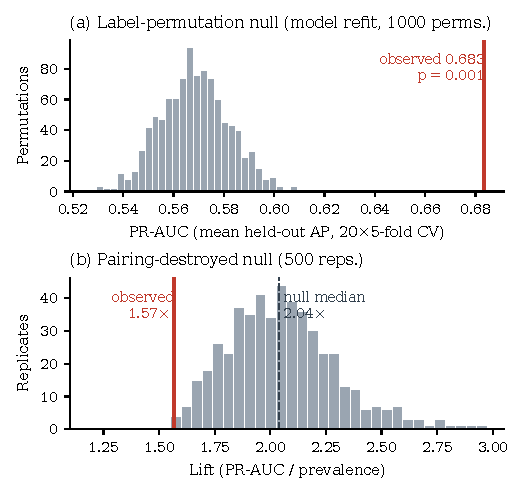
\includegraphics[width=\columnwidth]{figures/case1_nulls.pdf}
\caption{Story 1, original design. (a) Permutation null, with training
labels permuted inside each fold and the model refitted: the model passes. (b) Pairing-destroyed null
of lift, computed with the unfitted scorer (median 2.04$\times$; refitting
the full model on each shuffle gives a median of 1.99$\times$): the model
does not clear it. This null is conservative, so failing to clear it means
only that no response beyond regression to the mean has been shown, not that
none exists.}
\label{fig:case1}
\end{figure}

\begin{figure}[t]
\centering
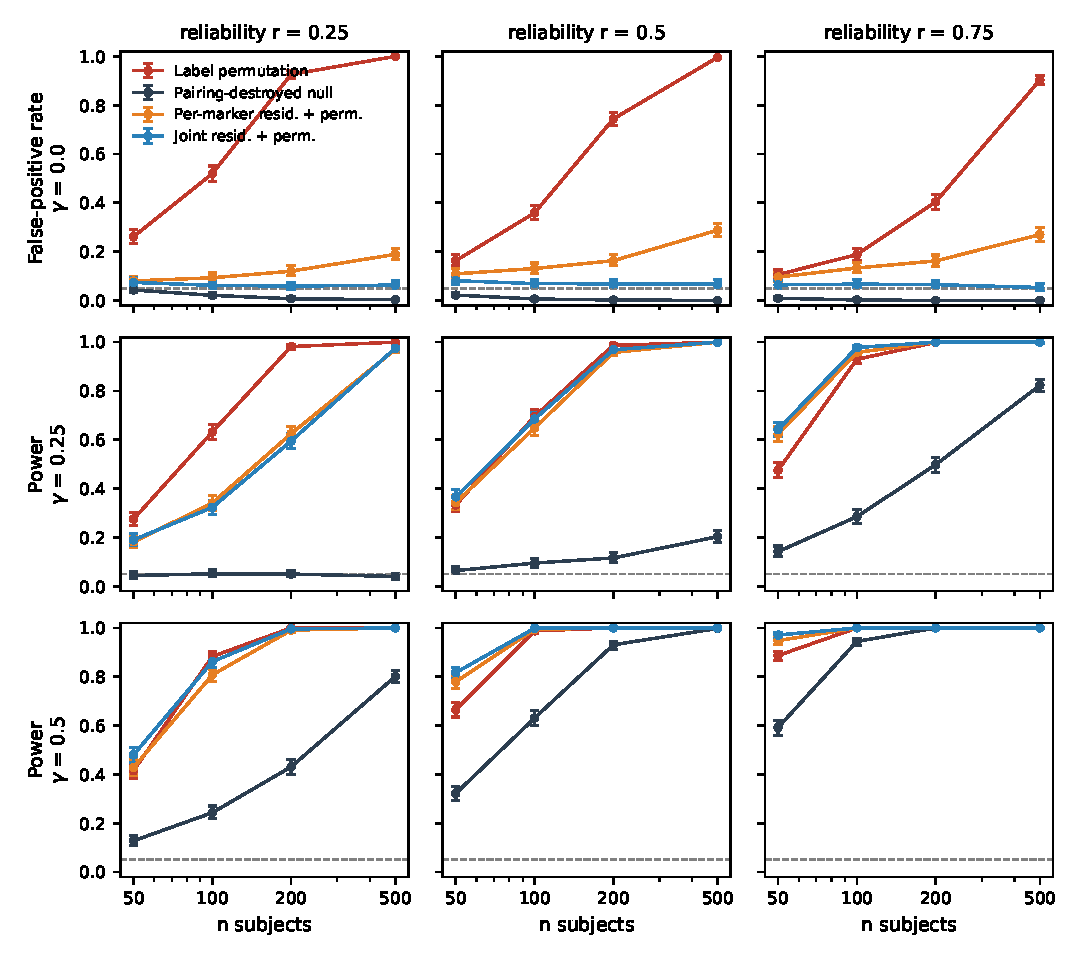
\includegraphics[width=\columnwidth]{figures/sim_rejection.pdf}
\caption{Simulated rejection rate against the number of subjects, 1{,}000
datasets per point. Top row: no forecastable response, so any rejection is a
false signal of forecasting skill. On raw change, label permutation rises
towards 100\% as $n$ grows because of coupling. Per-marker correction also
rises, because correlated markers leave residual coupling. Joint correction
stays at 5--8\%, close to the nominal rate plus a small excess. Columns:
measurement reliability. Dashed line: $\alpha=0.05$.}
\label{fig:sim}
\end{figure}

\subsection{The explanation that was faithful to the wrong thing}
\label{sec:story2}

\emph{What we believed.} A classifier separating preoperative from
twelve-month samples (PR-AUC 0.973, CV grouped by patient) relied on
metabolites that tell us how surgery changes metabolism, and ROAR confirmed
which ones.

\emph{Why the check passed.} Removing the SHAP-ranked features one at a time
and retraining hurt the model more than removing random features, from the
third removal on. ROAR was right: the model relied on those features. But the
first five removed included dimethyl sulfone, isopropanol and methanol.
Isopropanol is used for skin preparation, and handling during collection can
introduce exogenous compounds into samples \cite{bernini2011, vandersar2015};
these sources describe the general risk, not contamination of this cohort.
Dimethyl sulfone is a normal plasma metabolite that comes from diet, gut
bacteria and the body's own sulfur metabolism \cite{engelke2005}, any of
which could differ before and after surgery. We therefore call the three
\emph{putatively exogenous}. The deposited data cannot settle their origin,
and the argument below does not depend on it.

\emph{What we found.} Removing these three gave PR-AUC 0.954; removing three
established metabolites gave 0.959. Both removals reduced performance below
almost all random removals; the observed gap was 0.0056, against a
fold-to-fold standard deviation of about 0.03, and we performed no formal
equivalence test. ROAR, in other words, gave no sign that one group was
biology and the other was not. To avoid depending on the identity of any
real compound, we then added a synthetic feature equal to a multiple of the
label plus noise, with no biology at all. At an effect size similar to
dimethyl sulfone's, SHAP ranked it first in 6 of 10 draws and second in the
rest, and its median single-removal drop exceeded that of every real
metabolite. One caveat applies: SHAP rankings were computed on all 177
samples, including those later used for evaluation, so the informed
removals are subject to selection bias of unquantified magnitude
\cite{varma2006}. We therefore treat the ROAR comparisons as exploratory;
the synthetic feature supports the conceptual point without them.

\emph{The lesson.} A faithfulness test measures how much non-redundant signal
a feature carries, whatever its source. It is faithful to the model, and the
model is faithful to whatever separates the classes
\cite{adebayo2018, kumar2020}. ROAR cannot tell us whether the top features
are biology; for these three compounds the biological reading is
unsupported. The control that would have shown this is a feature known to
carry no biology, run through the same pipeline.

\subsection{The cohort that was two studies}
\label{sec:story3}

\emph{What we believed.} Urine NMR spectra separate people with type 2
diabetes from controls with PR-AUC 0.976, under CV grouped by subject.

\emph{Why the check passed.} Grouping by subject stops the model from
recognising a person it has already seen. It cannot detect a difference
shared by every member of a class.

\emph{What we found.} The 0.976 came from one random seed; over 20 seeds the
mean was 0.911 (range 0.845--0.975). We then cross-tabulated the label
against all 64 columns of the deposited metadata. Fifty-six were constant,
and apart from per-sample identifiers only sex and the label varied; no column recorded a date, batch or
run order. The deposited protocol, however, described two different
studies: 12 volunteers aged 18--55 sampled at seven fixed times, and patients
aged 30--65 with higher body-mass index sampled one to three times. Every
control sample name began with \texttt{ADG19007u} and every patient sample
name with \texttt{ADG10003u}. Age, body-mass index, sampling schedule and any
difference in how the two studies collected and stored urine are therefore
aliased with the label, and none is recorded per sample.

One methodological limit of our own audit belongs here. Which samples come
from which patient is not deposited, so we grouped patient samples with a
numbering heuristic. It merged at least three pairs of distinct patients,
which is conservative for those pairs, but we cannot rule out that it also
split one patient's samples across groups. Grouping does change the score:
over the same 20 seeds, grouped CV gave 0.911 (0.906 under an alternative,
stricter grouping) and ungrouped CV 0.969. The protocol problem, however,
does not depend on grouping: it is a property of the study design, and no
choice of folds can remove it.

\emph{The lesson.} The classifier may have learned diabetes, collection
protocol, or both; these data cannot tell which, because each protocol
contains only one class \cite{leek2010}. The disease interpretation is not
wrong so much as unidentifiable. The test that exposes this is not
statistical: read how each class was collected.

\subsection{The label that was named for something else}
\label{sec:story4}

\emph{What we believed.} Serum NMR separates obese from non-obese people with
ROC-AUC 0.960.

\emph{Why the check passed.} CV grouped by patient gave 0.960 and ungrouped CV
0.959. The agreement looked reassuring: no leakage between repeated samples.

\emph{What we found.} The ``non-obese'' class was the twelve-month
post-surgery visit of the same cohort. Of the 106 patients, 71 appear in both
classes and supply 80\% of the samples. The metadata record no body-mass
index, so we cannot check whether any twelve-month patient was non-obese.
The score reflects whatever differs between a person before bariatric
surgery and the same person a year later: weight loss, but potentially also
diet, supplements and medication after surgery, and a year's difference in
sample storage. These data cannot attribute it to obesity.

\emph{The lesson.} The correct name is ``pre- vs.\ post-surgery
classification.'' The check that catches a misnamed label is to write, in
one sentence, what physically distinguishes the two classes, and to compare
that sentence with the paper's title.

% ===========================================================================
\section{Why Passing Feels Like Proving}
\label{sec:why}

Looking back, the four failures share a structure. In each, the check
correctly established that the data contained predictive structure. What it
could not establish was where that structure came from: from the arithmetic
of the outcome, from compounds of uncertain origin, from the collection
protocol, or from surgery. Each of these rivals would pass the check as
easily as the biology we had in mind, so passing could not distinguish them.

Three habits made this easy to miss.

\emph{We reported checks, not rivals.} A methods section lists the checks
that were run. It rarely lists the alternative explanations those checks were
meant to exclude. Once a check is listed, it reads as a general certificate
of validity, though it excludes only one alternative. Reporting guidelines
already ask authors to define the outcome and its relation to the predictors
\cite{collins2024}; the step we skipped was asking which rival each check
answers.

\emph{We trusted bigger numbers more.} A smaller $p$-value, a larger $n$, or
an AUC near 1 feels like stronger evidence. Story~1 shows a setting in which
more data produced a more confident but equally uninformative rejection, and
Story~3 one in which a high, seed-dependent score sat on top of a design
confound. In small cohorts, a score close to 1 is a reason to look for a
proxy, not a reason to stop.

\emph{We checked the model, not the label.} All our checks took the label as
given. Two of our four failures were in the label itself (Stories~1 and 4),
and a third (Story~3) was in how its classes were collected. No amount of
model validation reaches a problem that sits upstream of the model.

These are not new statistical facts. Regression to the mean has been
described since at least 1962 \cite{oldham1962}, batch confounding is
well known in omics \cite{leek2010, han2022}, and leakage of many kinds has
been catalogued across ML-based science \cite{kapoor2023}. What our cases add
is that each passed a check that is commonly treated as sufficient, in work
by analysts who knew of the problem in general and did not recognise it in
their own data.

% ===========================================================================
\section{What We Do Now}
\label{sec:practice}

We now begin by naming the rival explanations for a headline score, and only
then choose the tests. For small-$n$ metabolomics we ask six questions; the
companion paper gives reference code for each \cite{vyw}.

\begin{enumerate}
  \item \emph{Is the outcome computed from the features?} If so, a label
        permutation is not evidence of a forecast. If the scientific target
        is change beyond what baseline predicts, regress change on
        \emph{all} baselines inside each training fold; if baseline-dependent
        change is itself of interest, this correction removes it, and a
        design with repeated baseline measurements is needed instead. In
        either case, report a pairing-destroyed null as a one-sided
        diagnostic.
  \item \emph{Was the model refitted inside every permutation, and is the
        permutation scheme stated?} If the observed statistic sits below
        the whole null, audit the null construction, the scoring pipeline,
        the model constraints and the fitting procedure before reading the
        $p$-value.
  \item \emph{Does the model beat a score that learns nothing?} Report the
        gap with an interval that resamples subjects.
  \item \emph{Could any feature come from sample handling or drugs?} Report
        results with and without such features, and run a feature known to
        carry no biology through the attribution pipeline.
  \item \emph{Does any metadata column or collection protocol line up with
        the label?} Cross-tabulate the label against every column and read
        how each class was collected.
  \item \emph{What, in one sentence, physically distinguishes the two
        classes?} If the sentence differs from the title, change the title.
\end{enumerate}

None of these questions needs new data. Applied to our own work, they change
what each analysis can claim. The responder forecast shows no evidence of
improvement over an unfitted score at $n=71$; this is absence of evidence,
not evidence that no forecast is possible. The ROAR study shows which
features the model relies on, not which are biology. The diabetes
classifier's disease interpretation cannot be separated from collection
protocol on these data. The obesity classifier is a pre- vs.\ post-surgery
classifier.

% ===========================================================================
\section{What We Are Not Claiming}
\label{sec:limits}

We audited our own analyses of three small public datasets, chosen because
their problems can be verified from the published files. We make no claim
about how common these failures are in the literature. Our findings concern
validation practice and say nothing for or against the biology of obesity,
bariatric surgery or diabetes. We have not shown that any classifier used
\emph{only} an artefact; we have shown that the checks could not rule the
artefact out. The exogenous origin of the compounds in Story~2 is plausible
but not established. The simulation behind Story~1 uses Gaussian data, a
linear model and one outcome rule, and the joint correction it supports also
removes any true dependence of change on baseline. The checks we discuss are
necessary; our point is only that they are not sufficient.

% ===========================================================================
\section{Conclusion}
\label{sec:conclusion}
Each of our four analyses passed its corresponding check, and in each the
check detected real predictive structure while the biological
interpretation we attached to it was unsupported or unidentifiable. A check
that passes tells you that one rival explanation has been excluded, not that
the interpretation is right. We suggest that small-cohort ML studies state
which rivals they have excluded, show the test that excluded each, and say
plainly which rivals remain open.

% ===========================================================================
\section*{Data and Code Availability}
MTBLS242, MTBLS1 and MTBLS881 are public through MetaboLights \cite{haug2020}.
All analyses, the simulation and a \texttt{RESULTS.md} listing every number
with its script, seed and command are in
\url{https://github.com/Calvinkub/validated-yet-wrong} (tag \texttt{paper-v1}).

\section*{Acknowledgment}
The authors thank Asst.\ Prof.\ Dr.\ Nont Kanungsukkasem, School of
Information Technology, King Mongkut's Institute of Technology Ladkrabang, for
advising this work. This research received no specific funding.

\section*{Use of Generative AI}
The authors used Claude (Anthropic) to assist with analysis code, the
simulation, and drafting text. The authors are responsible for the content
of this paper.

% ===========================================================================
\begin{thebibliography}{00}
\bibitem{vyw} C. Orrudee and K. C. Shomwiwat, ``Validated, yet wrong: Four ways small-$n$ metabolomics machine learning passes standard checks,'' draft, 2026. [Online]. Available: \url{https://github.com/Calvinkub/validated-yet-wrong}
\bibitem{repo_forecast} K. C. Shomwiwat, ``mtbls242-forecast-honest: corrected MTBLS242 forecast code and controls,'' GitHub, branch honest-evaluation, commit 637a58e, 2026. [Online]. Available: \url{https://github.com/Calvinkub/mtbls242-forecast-honest}
\bibitem{repo_roar} C. Orrudee, ``ROAR: remove-and-retrain analysis on MTBLS242,'' GitHub, commit f220cd2, 2026. [Online]. Available: \url{https://github.com/Chaiporn2005/ROAR}
\bibitem{repo_bridge} K. C. Shomwiwat, ``Bridge\_ai\_summit\_nmr\_2026: metabolic screening experiments,'' GitHub, commit 0088e38, 2026. [Online]. Available: \url{https://github.com/Calvinkub/Bridge_ai_summit_nmr_2026}
\bibitem{ojala2010} M. Ojala and G. C. Garriga, ``Permutation tests for studying classifier performance,'' \textit{J. Mach. Learn. Res.}, vol. 11, pp. 1833--1863, 2010.
\bibitem{hooker2019} S. Hooker, D. Erhan, P.-J. Kindermans, and B. Kim, ``A benchmark for interpretability methods in deep neural networks,'' in \textit{Proc. Adv. Neural Inf. Process. Syst. (NeurIPS)}, vol. 32, 2019.
\bibitem{haug2020} K. Haug \textit{et al.}, ``MetaboLights: a resource evolving in response to the needs of its scientific community,'' \textit{Nucleic Acids Res.}, vol. 48, no. D1, pp. D440--D444, Jan. 2020, doi: 10.1093/nar/gkz1019.
\bibitem{mtbls242} EMBL-EBI, ``MetaboLights study MTBLS242: Metabolomic fingerprint of severe obesity is dynamically affected by bariatric surgery in a procedure-dependent manner,'' dataset. [Online]. Available: \url{https://www.ebi.ac.uk/metabolights/MTBLS242}
\bibitem{gralka2015} E. Gralka, C. Luchinat, L. Tenori, B. Ernst, M. Thurnheer, and B. Schultes, ``Metabolomic fingerprint of severe obesity is dynamically affected by bariatric surgery in a procedure-dependent manner,'' \textit{Am. J. Clin. Nutr.}, vol. 102, no. 6, pp. 1313--1322, Dec. 2015, doi: 10.3945/ajcn.115.110536.
\bibitem{salek2007} R. M. Salek \textit{et al.}, ``A metabolomic comparison of urinary changes in type 2 diabetes in mouse, rat, and human,'' \textit{Physiol. Genomics}, vol. 29, no. 2, pp. 99--108, Apr. 2007, doi: 10.1152/physiolgenomics.00194.2006.
\bibitem{maltesen2020} R. G. Maltesen, R. Wimmer, and B. S. Rasmussen, ``A longitudinal serum NMR-based metabolomics dataset of ischemia-reperfusion injury in adult cardiac surgery,'' \textit{Sci. Data}, vol. 7, Art. no. 198, 2020, doi: 10.1038/s41597-020-0545-0.
\bibitem{barnett2005} A. G. Barnett, J. C. van der Pols, and A. J. Dobson, ``Regression to the mean: what it is and how to deal with it,'' \textit{Int. J. Epidemiol.}, vol. 34, no. 1, pp. 215--220, Feb. 2005, doi: 10.1093/ije/dyh299.
\bibitem{tu2007} Y.-K. Tu and M. S. Gilthorpe, ``Revisiting the relation between change and initial value: a review and evaluation,'' \textit{Stat. Med.}, vol. 26, no. 2, pp. 443--457, Jan. 2007, doi: 10.1002/sim.2538.
\bibitem{archie1981} J. P. Archie, ``Mathematic coupling of data: a common source of error,'' \textit{Ann. Surg.}, vol. 193, no. 3, pp. 296--303, Mar. 1981, doi: 10.1097/00000658-198103000-00008.
\bibitem{bernini2011} P. Bernini, I. Bertini, C. Luchinat, P. Nincheri, S. Staderini, and P. Turano, ``Standard operating procedures for pre-analytical handling of blood and urine for metabolomic studies and biobanks,'' \textit{J. Biomol. NMR}, vol. 49, no. 3--4, pp. 231--243, 2011, doi: 10.1007/s10858-011-9489-1.
\bibitem{vandersar2015} S. A. van der Sar \textit{et al.}, ``Ethanol contamination of cerebrospinal fluid during standardized sampling and its effect on $^1$H-NMR metabolomics,'' \textit{Anal. Bioanal. Chem.}, vol. 407, no. 16, pp. 4835--4839, Jun. 2015, doi: 10.1007/s00216-015-8663-9.
\bibitem{engelke2005} U. F. H. Engelke, A. Tangerman, M. A. A. P. Willemsen, D. Moskau, S. Loss, S. H. Mudd, and R. A. Wevers, ``Dimethyl sulfone in human cerebrospinal fluid and blood plasma confirmed by one-dimensional $^1$H and two-dimensional $^1$H--$^{13}$C NMR,'' \textit{NMR Biomed.}, vol. 18, no. 5, pp. 331--336, 2005, doi: 10.1002/nbm.966.
\bibitem{adebayo2018} J. Adebayo, J. Gilmer, M. Muelly, I. Goodfellow, M. Hardt, and B. Kim, ``Sanity checks for saliency maps,'' in \textit{Proc. Adv. Neural Inf. Process. Syst. (NeurIPS)}, vol. 31, 2018.
\bibitem{kumar2020} I. E. Kumar, S. Venkatasubramanian, C. Scheidegger, and S. Friedler, ``Problems with Shapley-value-based explanations as feature importance measures,'' in \textit{Proc. 37th Int. Conf. Mach. Learn. (ICML)}, PMLR vol. 119, 2020, pp. 5491--5500.
\bibitem{varma2006} S. Varma and R. Simon, ``Bias in error estimation when using cross-validation for model selection,'' \textit{BMC Bioinformatics}, vol. 7, Art. no. 91, 2006, doi: 10.1186/1471-2105-7-91.
\bibitem{leek2010} J. T. Leek \textit{et al.}, ``Tackling the widespread and critical impact of batch effects in high-throughput data,'' \textit{Nat. Rev. Genet.}, vol. 11, no. 10, pp. 733--739, Oct. 2010, doi: 10.1038/nrg2825.
\bibitem{han2022} W. Han and L. Li, ``Evaluating and minimizing batch effects in metabolomics,'' \textit{Mass Spectrom. Rev.}, vol. 41, no. 3, pp. 421--442, 2022, doi: 10.1002/mas.21672.
\bibitem{collins2024} G. S. Collins \textit{et al.}, ``TRIPOD+AI statement: updated guidance for reporting clinical prediction models that use regression or machine learning methods,'' \textit{BMJ}, vol. 385, Art. no. e078378, 2024, doi: 10.1136/bmj-2023-078378.
\bibitem{oldham1962} P. D. Oldham, ``A note on the analysis of repeated measurements of the same subjects,'' \textit{J. Chronic Dis.}, vol. 15, no. 10, pp. 969--977, 1962, doi: 10.1016/0021-9681(62)90116-9.
\bibitem{kapoor2023} S. Kapoor and A. Narayanan, ``Leakage and the reproducibility crisis in machine-learning-based science,'' \textit{Patterns}, vol. 4, no. 9, Art. no. 100804, Sep. 2023, doi: 10.1016/j.patter.2023.100804.
\end{thebibliography}

\end{document}
